% !TEX encoding = windows-1251
% !TEX program = pdflatex
\documentclass[11pt]{article}
\usepackage[cp1251]{inputenc}
%\usepackage[T2A]{fontenc}
%\usepackage[russian]{babel}
\usepackage{subcaption}
\usepackage{amssymb,amsmath}
\usepackage{multicol}
\pagestyle{empty}
\usepackage{graphicx}
\textheight=25cm
\textwidth=18cm
\oddsidemargin=-1cm
\topmargin=-2.5cm
\newtheorem{lem}{Lemma}
\DeclareMathOperator{\suff}{suff}
\DeclareMathOperator{\pref}{pref}
\DeclareMathOperator{\overlap}{overlap}

\begin{document}
	\begin{lem}
		Let $GHA(\mathcal{S})$ return a superstring corresponding to a permutation $\sigma = (s_{i_1}, s_{i_2}, \dots, s_{i_n})$. Then an algorithm $A$ that merges adjacent strings in $\sigma$ in the descending order of the lengths its overlaps is greedy.
	\end{lem}
	{\em Proof.} Let $c$ be a cycle through solution $D$ of $GHA(\mathcal{S})$ in the hierarchical graph and let us denote by $c_k$ a part of $c$ above level $k$ for any $k$. Since $c$ is a sequence of arcs
	\begin{gather*}
		\varepsilon \to \dots \to \pref(s_{i_1}) \to s_{i_1} \to \suff(s_{i_1}) \to \dots \to \overlap(s_{i_1}, s_{i_2}) \to \dots \to s_{i_2} \to \dots \to s_{i_n} \to \dots \to \varepsilon,
	\end{gather*}
	$c_k$ can be represented as disjoint union $\mathcal{P}_k$ of subsequences of $c$ (in other words, subpaths of $c$), such that any of them begins and ends on level $k$, but all its inner vertices are above level $k$ (fig. \ref{fig:1a} and \ref{fig:1b}).
	
	By construction of $c$ every such path $p$ contains at least one string from $\mathcal{S}$ and if it contains more than one string, then in $\sigma$ they go sequentially and in the same order in which $p$ visits them. This allows us to treat such paths as already constructed superstrings of the corresponding subsets of $\mathcal{S}$. From this point of view, we can naturally identify every merge of  some superstrings $s$ and $t$ with $|\overlap(s,t)| = k$ performed by $A$ with situation when for the corresponding paths $p_s, p_t \in \mathcal{P}_k$ there is a path $p \in \mathcal{P}_{k-1}$ containing $p_s \circ p_t$ as subpath (fig. \ref{fig:1c}). It is easy to see, that in general $s$ and $t$ can be merged only if the corresponding paths {\em touch}, i.e. a head vertex of $p_s$ is also a tail vertex of  $p_t$ (of course, this fact doesn't imply that this paths will be merged, as there, for example, may be another path $p_r \in \mathcal{P}_k$ such that $p_r$ and $p_t$ touch and there is $p \in \mathcal{P}_{k-1}$ which contains $p_r \circ p_t$). It is also clear, that if $A$ at some step doesn't merge a pair of superstrings $s, t$ with strictly maximal overlap of the length~$k$, then corresponding paths $p_s, p_t \in \mathcal{P}_k$ touch at some vertex $v$, but there are paths $p'_s, p'_t \in \mathcal{P}_{k-1}$ such that $p'_s$ ends with $p_s \circ (v, \suff(v))$ and $p'_t$ starts with $(\pref(v), v) \circ p_t$. In other words, $p_s$ isn't merged with any other path with start in $v$, $p_t$ isn't merged with any other path with end in $v$ and both are contained in the different paths in $\mathcal{P}_{k-1}$.
	
	In this way, it is sufficient to show that such situations don't happen, to prove that $A$ is greedy. Let us suppose the opposite and consider the mentioned paths $p_s$, $p_t$, $p'_s$, $p'_t$ and the vertex $v$. By definition of $v$ it has income down-arc and outgoing up-arc and also income up-arc and outgoing down-arc, which by construction of $D$ can be only in the case when $v$ is the last chance of the corresponding component $\mathcal{C} \ni v$ to be connected to the rest arcs in $D$. It immediately follows, that all component $\mathcal{C}$ (and hence the paths  $p_s$ and $p_t$) lies in some path $p_{\mathcal{C}} \in \mathcal{P}_{k-1}$, which contradicts the definition of $p'_s$ and $p'_t$. This contradiction completes the proof. $\square$
	
	\begin{figure}[h]
		\centering
		\begin{subfigure}[t]{0.45\textwidth}
			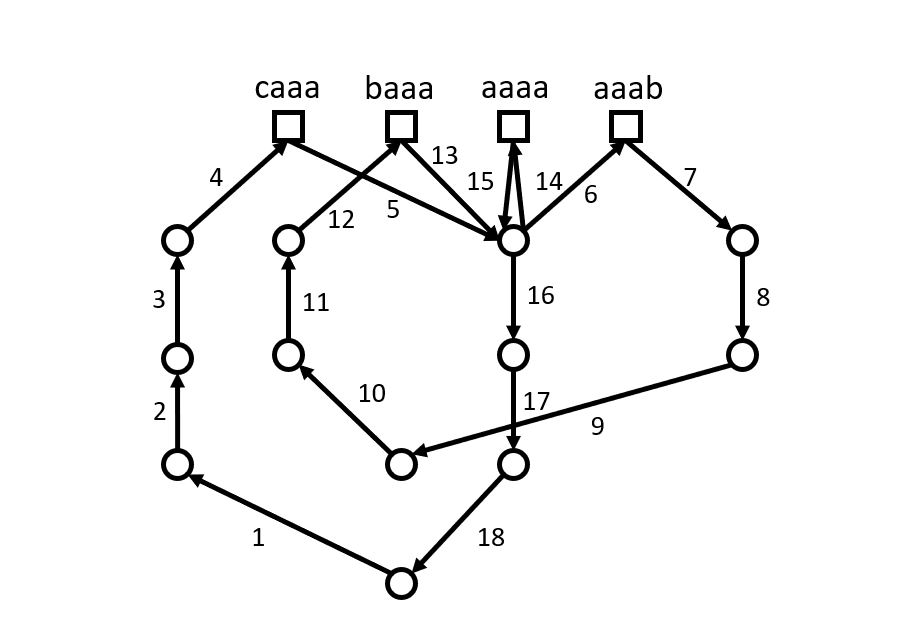
\includegraphics[width=\textwidth]{gha_is_greedy_img/fig1.png}
			\caption{Cycle $c$ for $\mathcal{S} = \{ {\tt aaaa, baaa, caaa, aaab} \}$. Numeration indicates an order of arcs and corresponds to solution $\tt caaabaaaa$.}
			\label{fig:1a}
		\end{subfigure}
		\hfil
		\begin{subfigure}[t]{0.45\textwidth}
			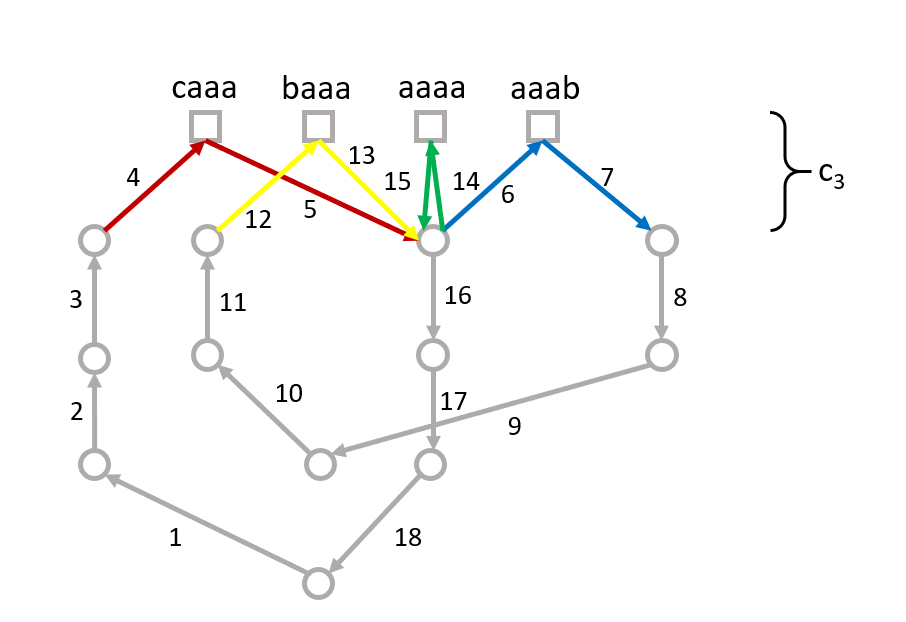
\includegraphics[width=\textwidth]{gha_is_greedy_img/fig2.png}
			\caption{Colored arcs is $\mathcal{P}_3$, which contains four paths painted in different colours. Note, that there are many opportunities for merging. For example, one can merge red, green and blue paths, and leave the yellow as is. This doesn't mean, however, that they will be merged --- everything is decided by the numeration.}
			\label{fig:1b}
		\end{subfigure}

		\begin{subfigure}[t]{0.45\textwidth}
			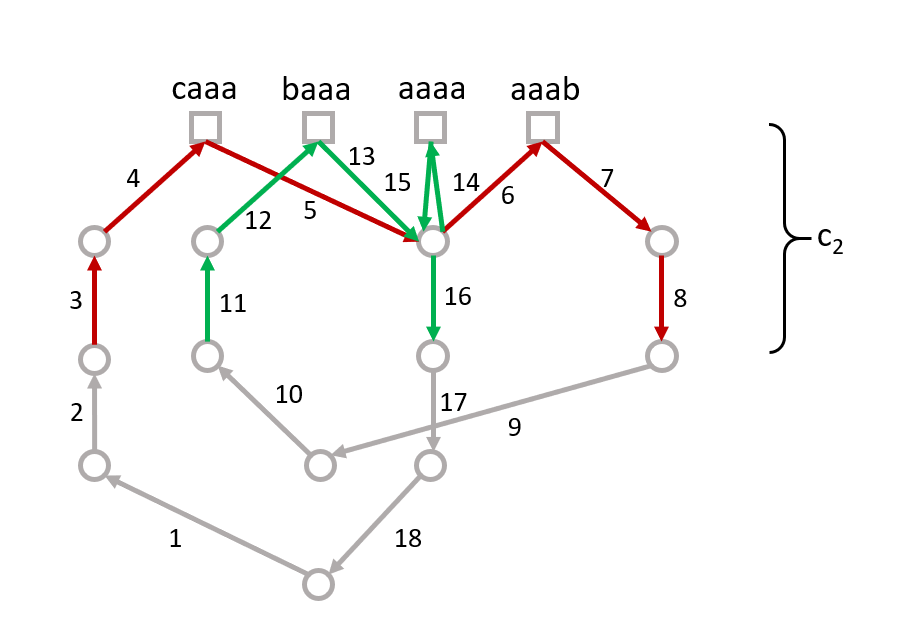
\includegraphics[width=\textwidth]{gha_is_greedy_img/fig3.png}
			\caption{Colored arcs is $\mathcal{P}_2$. We see, that red and blue paths from \ref{fig:1b} were merged and now are subpaths of red. It means, that $A$ merged strings {\tt caaa} and {\tt aaab}. The same goes for green path: merging of yellow and green paths from \ref{fig:1b} indicates, that $A$ merged {\tt baaa} and {\tt aaaa}}
			\label{fig:1c}
		\end{subfigure}
		\hfil
		\begin{subfigure}[t]{0.45\textwidth}
			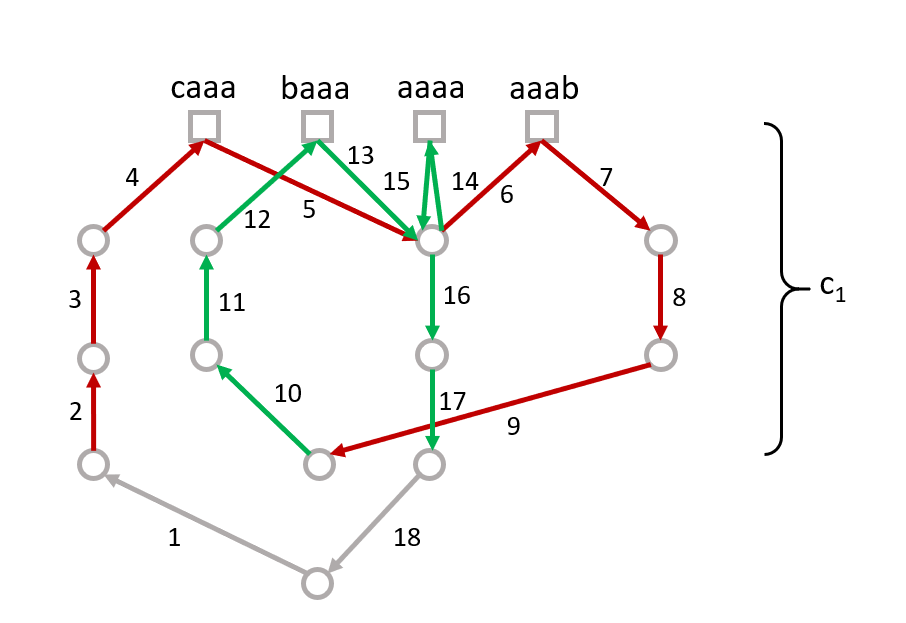
\includegraphics[width=\textwidth]{gha_is_greedy_img/fig4.png}
			\caption{Colored arcs is $\mathcal{P}_1$, which still contains two paths. This means, that there were not merges. It is easy to see, that in the next step $A$ will merge {\tt caaab} and {\tt baaaa} and there will be only one path coincides with $c$.}
			\label{fig:1d}
		\end{subfigure}
	\caption{}
	\end{figure}
	
\end{document}
